\section{Introduction} \label{sect:intro}

``What's in a name?" --- in the context of networking, quite a lot! IP addresses and prefixes
indicate to routers where particular interfaces or subnets reside in the greater Internet
\cite{bgp}. Domain
names offer a simple, human-readable overlay for the complicated, often multiplexed addressing
scheme underneath \cite{dns}. Autonomous system (AS) numbers often help to distinguish one network
from another \cite{asn}.
Names and labels such as these, whatever form they take, allow us to organize immense network spaces
with manageable and descriptive abstractions.

Unfortunately, a single name is often not enough. One machine can be described in terms of all of
the examples listed above, and more. This is because it is important that names carry information
relevant to the specific way in which they will be used. Routers are unable to direct traffic with
domain names, just as humans cannot be expected to remember the plethora IP addresses they access
every day. While it is intuitive that no labeling system is applicable across all possible
dimensions, in practice, this fact is often taken for granted or neglected entirely.

In this project, we challenge the careless application of conventional client labeling schemes in
Internet measurement experiments, particularly those subject to the effects of DNS redirection and
CDN PoP (point of presence) catchment formation. We uncover and quantify the degree of misalignment
between experimentally determined aggregate catchments and labels often assumed to indicate
``similarity" between clients --- country, AS number, announced BGP prefix, and /24 subnet --- and
use this to design the Skyline model, a grouping system which describes clients' relative distances
from each other in terms of their \emph{common network resource exposure} (CNRE). Describing clients in such
terms highlights what should be a chief concern in large scale Internet measurement platforms and
network optimization efforts: the sets of clients actually being directed to the same resources.

\begin{figure*}
    \center
        \mbox{
            \begin{subfigure}[b]{0.5\linewidth}
                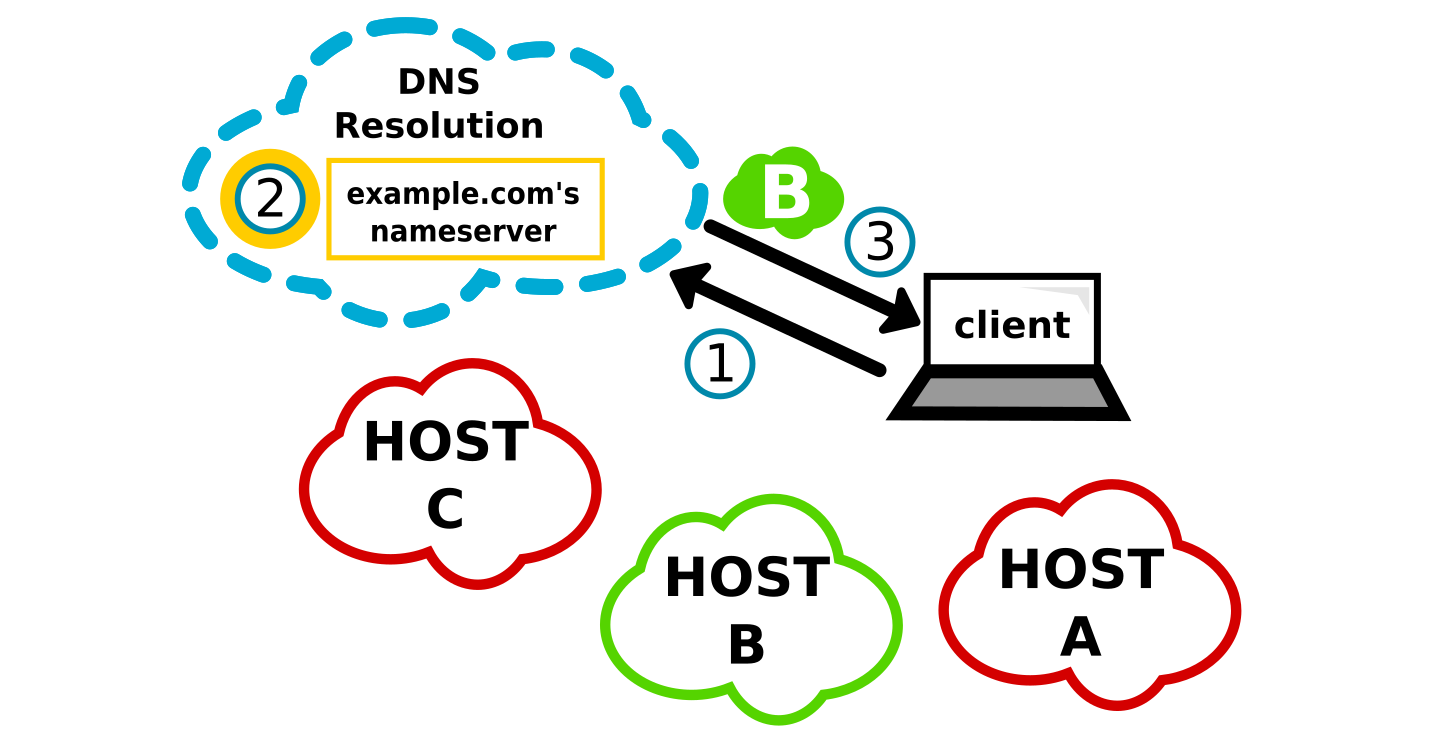
\epsfig{file=figs/dns_resolution.png, width=1\linewidth}
                \caption{\label{fig:dns}}
            \end{subfigure}
            \begin{subfigure}[b]{0.5\linewidth}
                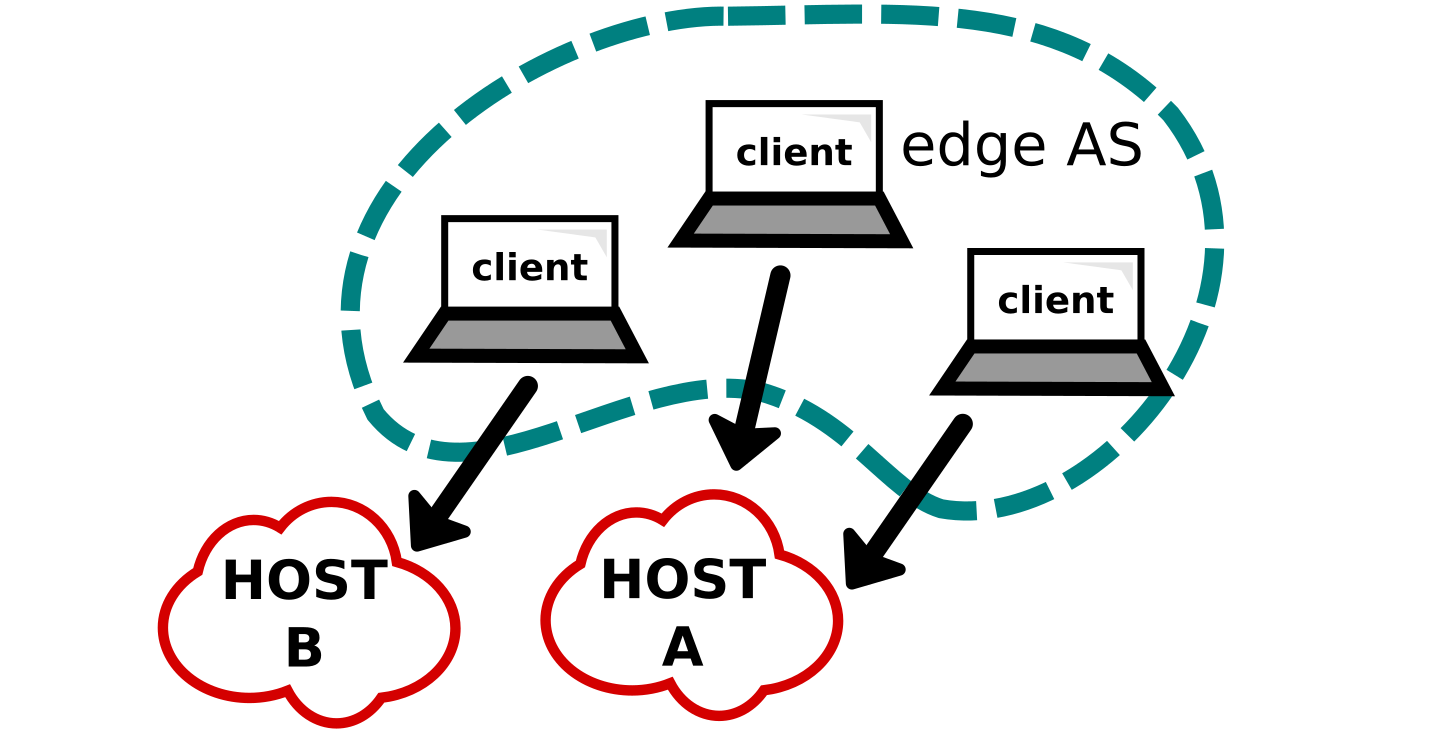
\epsfig{file=figs/client_mapping.png, width=1\linewidth}
                \caption{\label{fig:mismatch}}
            \end{subfigure}
        }
    \caption{
        Illustration of network resource allocation. Figure \ref{fig:dns} shows DNS resolution at a high level: 1)~The client deploys a DNS query for example.com. 2) This query ultimately reaches nameserver responsible for example.com and decides which of example.com's network resources should serve the client. 3) The nameserver's resource selection is returned to the client. Figure \ref{fig:mismatch} shows an example of how clients with similarly described locations may
        be directed to distinct network resources.
    }
\end{figure*}

In order to develop the Skyline model, we performed an exhaustive set of measurements to frame
client experience on a per \emph{site} basis. In this work, we capture a
snapshot of both DNS resolutions and latency measurements toward the 304 domains that appeared most
frequently in the top 2441 most popular webpages. Our measurements span over 10,000 unique
clients spread across 185 countries and 3637 autonomous systems. We performed over 52 million pairwise
comparisons with the results of these measurements to arrive at the foundation of what we have
coined the ``Skyline model". 

This paper makes the following contributions: %, including those we expect to stem from
%proposed work, which we have designated with (\emph{p})

\begin{itemize}%\parskip0pt \parsep0pt
    \item We perform a large exploration of client network performance on a per webpage level. Our
        raw results are publicly available on the RIPE Atlas platform.
    \item  We quantify the degree of misalignment between conventional grouping schemes
        and aggregate catchments.
    \item  We introduce the Skyline model, a client grouping scheme that reflects the
        extent of CNRE.
    \item  Using the Skyline model, we identify and analyze network resource islands --- 
        sets of clients with very high degrees CNRE. 
\end{itemize}

% RELATED WORK and PROBLEM FRAMING
\section{Problem Space and Related Work} \label{skyspace}

This projects aims to gain an understanding of which clients are directed to the same set of
resources across many distinct domains. Its most direct and immediate use case is influencing probe
selection in large scale Internet measurements. For researchers, likely unaware of the relatively
hidden allocation schemes of the wide array of CDN platforms and other large content distributors,
it is difficult to determine, a priori, the degree of similarity between clients. Knowledge of
whether there is a high probability that a pair of clients are being directed to altogether
different resources may be significant to their experiment design. This approach to experiment
design is in line with RIPE Atlas, one of the largest client based measurement platforms,
which maintains
an exhaustive set of tags on all of their clients in order to help researchers and network operators
filter and refine the set selected for their experiment \cite{ripe-atlas}. Further, more abstract
applications may include, but are not limited to, distributed denial of service mitigation
\cite{anycastvsddos} and CDN node deployment \cite{35590, Tariq}.

The most similar body of related work involves anycast CDN catchment analysis, which aims to
investigate the set of clients routed towards particular CDN points of presence (PoPs)
\cite{Calder2015, anycastvsddos, vdmscatchment}. Our work differs significantly in scope: to our 
knowledge, we are the first to investigate what we refer to as \emph{aggregate catchments}, the joint
behavior of many anycast CDN catchments and unicast CDN targets, spread across many content
distribution platforms. Conversely, this related body work either focuses on individual platforms or
specific services \cite{Calder2015, anycastvsddos, vdmscatchment}. 

Several authors have attempted to discover the topology of large CDN platforms through large scale
measurement studies \cite{webcart, Calder2013, benson11}. While their findings are potentially of
use in this project, their goals and contributions run parallel to what we aim to accomplish. They
seek to identify the properties and locations of CDN resources; conversely, we seek to identify the
target pools (sets of clients) of overlapping CDN resource catchments \cite{webcart, Calder2013,
benson11}. Other work close to this space investigates the performance of a particular CDN
deployment scheme \cite{ecs15sigcomm}.
